\documentclass[a4paper,10pt]{article}
\usepackage[utf8]{inputenc}
\usepackage[pdftex]{graphicx}

%opening
\title{LaTex Model 01\\---``How do I include tables and figures?''---}
\author{A.M. Roma}

\begin{document}

\maketitle

\begin{abstract} In the following examples, we show how to include some floats such as tables and figures in your LaTex document. Exercise: If written in Portuguese, you must use the words {\it Março}, {\it Resumo}, {\it Tabela}\, e {\it Figura} instead of their English counterparts. How can you get this done? Share your knowledge via {\it Fórum do Estudante}.\end{abstract}

%%%%%%%%%%%%%%%%%%%%%%%%%%%%%%%%%%%%%%%%%%%%%%%%%%%%%%%%%%%%%%%%%%%%%%%%%%%%%
\section{Inclusão de Tabela}
A Tabela~\ref{tabmodel-1} foi confeccionada para analisar a convergência do Método de Euler no instante $t=T$ 
de uma sequência de aproximações numéricas calculadas por este método, $\eta(T,h_n)$, para a solução exata $y(T)$, à medida que usa\-mos passos de integração progressivamente menores, $h_n$. Esta análise é baseada  observando-se o comportamento do valor absoluto do {\it erro de discretização global}, 
$\left|e(T, h_n)\right|=\left|y(T)-\eta(T,h_n)\right|,$ reportado na terceira coluna da Tabela~\ref{tabmodel-1}.

\begin{table}[!ht]
\centering
\begin{tabular}{rccc}\hline\hline\\
 $n$ &$h_n=\displaystyle \frac{(T-t_0)}{n}$ & $\left|e(T, h_n)\right|$  & ordem $p$\\\\
	\hline\hline
	\\
  128 &  1.95312e-03 &  1.30556e-11 &  ----------- \\
  256 &  9.76562e-04 &  1.01275e-11 &  3.66390e-01 \\
  512 &  4.88281e-04 &  6.49856e-12 &  6.40090e-01 \\
 1024 &  2.44141e-04 &  3.70427e-12 &  8.10930e-01 \\
 2048 &  1.22070e-04 &  1.98031e-12 &  9.03467e-01 \\
 4096 &  6.10352e-05 &  1.02417e-12 &  9.51272e-01 \\
 8192 &  3.05176e-05 &  5.20845e-13 &  9.75525e-01 \\
16384 &  1.52588e-05 &  2.62646e-13 &  9.87736e-01 \\
		\hline\hline
\end{tabular}
\caption{Método de Euler aplicado ao Problema de Cauchy em $t=T$. 
}
\label{tabmodel-1}
\end{table}
\section{Including figures}
Peskin received an A.B. (1968) from Harvard University and a Ph.D. (1972) from the Albert Einstein College of Medicine, Yeshiva University and shortly thereafter joined the faculty of the Courant Institute of Mathematical Sciences, New York University. Figures~\ref{peskin}, \ref{peskin&heart}, and \ref{double} show how figures are inserted in the text (find out how to make it write ``Figura'')


\hspace{0.1pc}

\begin{figure}
\begin{center}
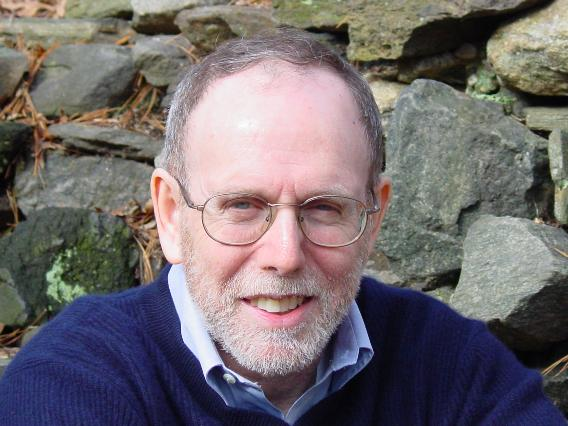
\includegraphics[scale=0.205]{figures/DSC01508_scale4.jpeg}
\end{center}
\caption{Peskin and his 3D heart model.}
\label{peskin}
\end{figure}

\begin{figure}
\begin{center}
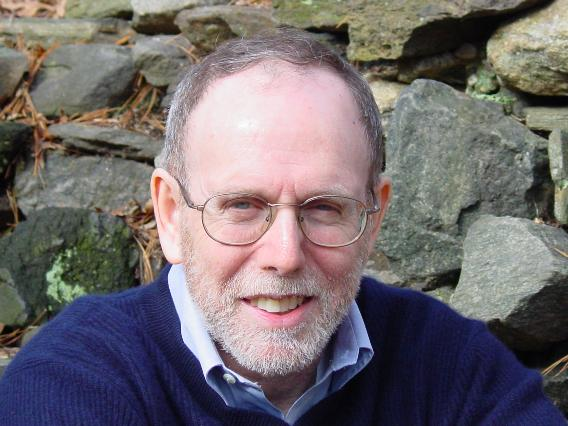
\includegraphics[scale=0.205]{figures/DSC01508_scale4.jpeg}
\hspace{0.1pc}
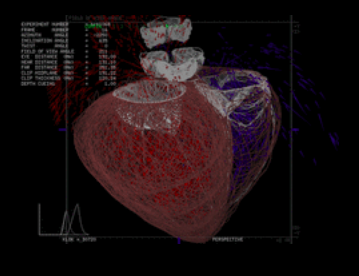
\includegraphics[scale=0.32]{figures/3D heart.png}
\end{center}
\caption{Peskin and his 3D heart model.}
\label{peskin&heart}
\end{figure}

\begin{figure}
\begin{center}
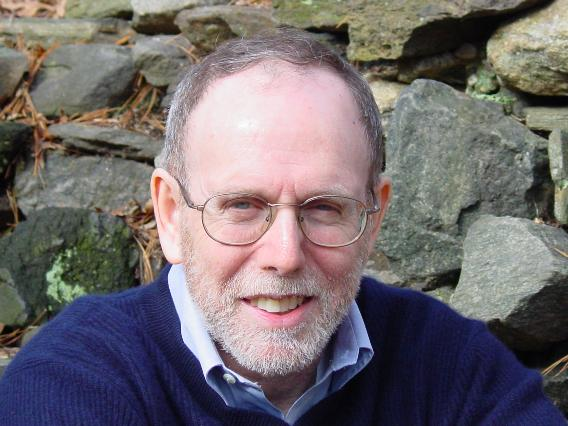
\includegraphics[scale=0.205]{figures/DSC01508_scale4.jpeg}
\hspace{0.1pc}
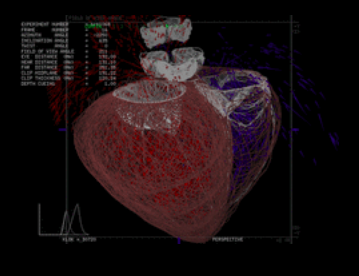
\includegraphics[scale=0.32]{figures/3D heart.png}\\
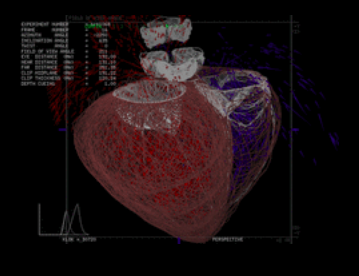
\includegraphics[scale=0.32]{figures/3D heart.png}
\hspace{0.1pc}
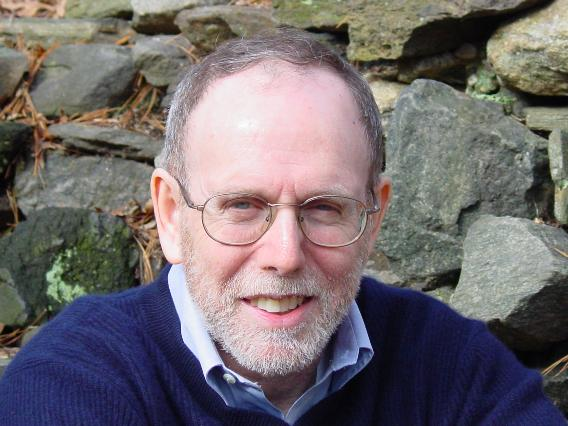
\includegraphics[scale=0.20]{figures/DSC01508_scale4.jpeg}
\end{center}
\caption{Peskin and his 3D heart model.}
\label{double}
\end{figure}




\end{document}
